\chapter{Solving for Neutrino Longitudinal Momentum}
\label{app:nupz_studies}

Neutrinos are not detected directly using the ATLAS detector. Instead, their transverse momentum is determined using conservation of momentum. The longitudinal momentum of neutrinos can be calculated in terms of the momentum and masses of other particles in the event, but it is a solution to a quadratic equation, and hence there are two possible solutions. Please see Sec.~\ref{sec:selection} for the equations. We investigated the efficiencies of several different methods of picking the solution.

Several methods for selecting the sign were tested on truth level using the signal Monte Carlo samples for resonant diHiggs production with mass of 700 GeV, 2000 GeV and 5000 GeV. The choice of sign is said to be correct if the solution is within 10$\%$ of the truth value if the truth value is larger than 100 GeV or within 10 GeV if the truth value is smaller than 100 GeV. This criterion was chosen to take into account the fact that we do not need to know the exact momentum, just the momentum up to errors from the detector resolution. 

\subsection{$W$ mass method}
The mass of the $W$ that decays leptonically can be calculated from the momentum of the lepton and neutrino since $P_{W} = P_{l} + P_{\nu}$. The mass of the leptonic $W$ we calculate with the chosen solution depends on our choice of sign. As figure \ref{fig:wdist} shows, the $W$ mass distribution has peaks at 40 and 80 GeV. So for this method, we will use the solution that minimises $|m_{W} - 80|$ or $|m_{W} - 40|$.

\begin{figure}[!h]
\begin{center}
\includegraphics*[width=0.47\textwidth] {figures/nupz/wmassdist.png}
\includegraphics*[width=0.47\textwidth] {figures/nupz/wmass700.png}
	\caption{$m_{W}$ Distribution and the solution using $W$ mass method.}
\label{fig:wdist}
\end{center}
\end{figure}

\subsection{$\eta$ solution}
The next method we tested was picking the sign in the solution that is the opposite of the sign of $\eta$ of the lepton. This was motivated by studying the same problem for single $W$ production and noticing that there is a correlation between the the correct sign choice and the sign of $\eta$. This correlation is shown in figure \ref{fig:etaplots}. It is interesting to note that this method is mathematically equivalent to using the opposite sign of the longitudinal momentum of the lepton. This can be verified by looking at the definition of $\eta_{l} = \frac{1}{2} \log \frac{p_{l} + p_{l,z}}{p_{l} - p_{l,z}}$. If $p_{l,z} < 0$ then $\frac{p_{l} + p_{l,z}}{p_{l} - p_{l,z}} < 1$ so $\eta_{l} < 0$ and similarly if $p_{l,z} > 0$ then $\eta_{l} > 0$. 

We also tested using the opposite sign of $\eta$ of the $l q \bar{q}$ system. Using the additional information from the quark antiquark pair allows us to pick the correct sign more often than just using $\eta_{l}$, ~\ref{fig:etalqqplots}
\begin{figure}
		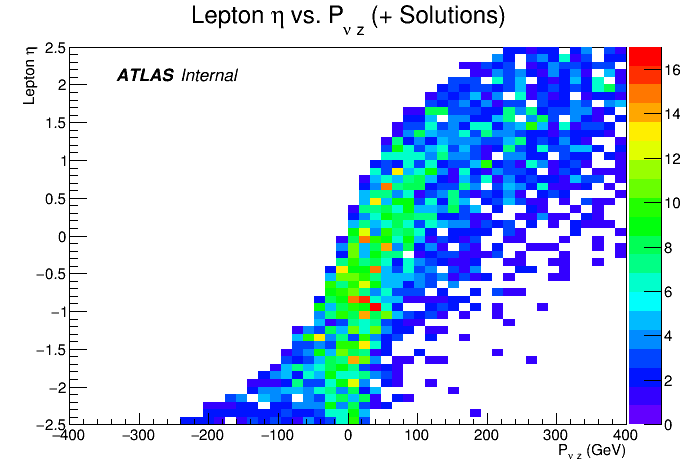
\includegraphics[width=0.47\textwidth]{figures/nupz/wminus.png}
		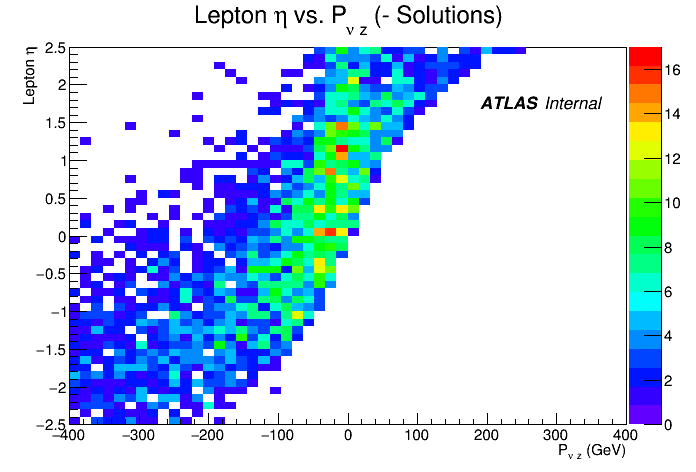
\includegraphics[width=0.47\textwidth]{figures/nupz/wplus.png}
		\caption{Single $W$ $\eta_{l}$ vs Correct Sign Choice}
		\label{fig:etaplots}
\end{figure}

\begin{figure}[!h]
\begin{center}
\includegraphics*[width=0.47\textwidth] {figures/nupz/etaldist.png}
\includegraphics*[width=0.47\textwidth] {figures/nupz/eta-l700.png}
	\caption{$\eta_{l}$ and the solution using $\eta_{l}$ method in 700 GeV resonant sample.}
\label{fig:wdist}
\end{center}
\end{figure}

\begin{figure}[!h]
\begin{center}
	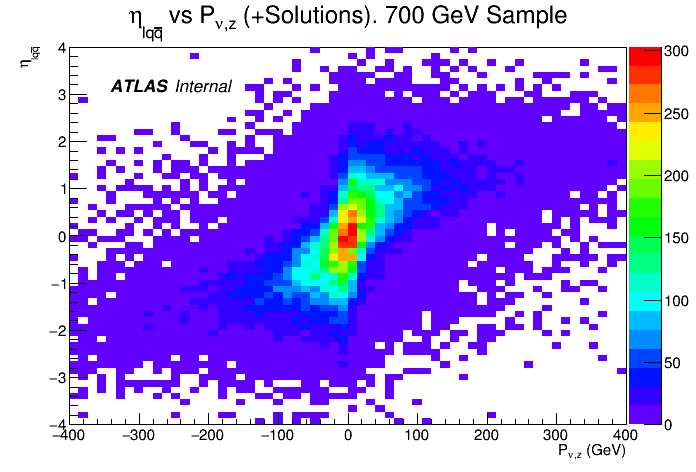
\includegraphics[width=0.47\textwidth]{figures/nupz/etalqqplus.png}
	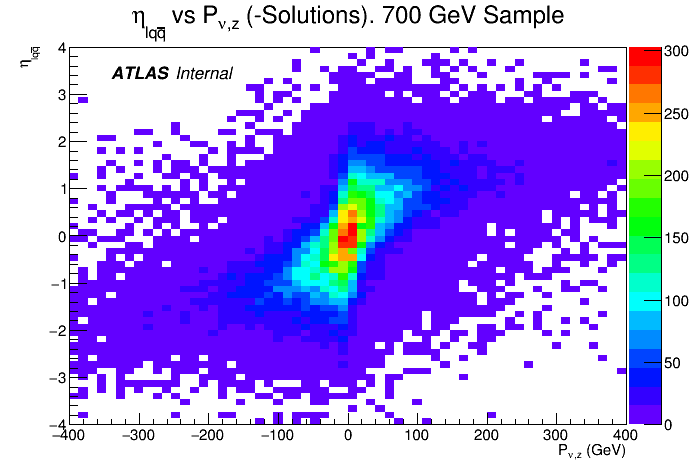
\includegraphics[width=0.47\textwidth]{figures/nupz/etalqqminus.png}
	\caption{Higgs pair $\eta_{l q \bar{q}}$ vs Correct Sign Choice}
	\label{fig:etalqqplots}
\end{center}
\end{figure}

\begin{figure}[!h]
\begin{center}
\includegraphics*[width=0.47\textwidth] {figures/nupz/etalqqdist.png}
\includegraphics*[width=0.47\textwidth] {figures/nupz/eta-lqq700.png}
	\caption{$\eta_{l}$ and the solution using $\eta_{l}$ method in 700 GeV resonant sample.}
\label{fig:etaplots}
\end{center}
\end{figure}

\subsection{$\Delta$ R Method}
We also investigated minimising $\Delta R(l,\nu)$.  This is motivated by the idea that the neutrino and the charged lepton produced from the same $W$ should be near each if the $W$ boson is boosted, which is often the case for heavy resonances decaying into $W$ boson. Fig.~\ref{fig:deltaRsolution} shows the $\Delta R(l,\nu)$ and the solution using $\Delta R(l,\nu)$ method in 700 GeV resonant sample.

\begin{figure}[!h]
\begin{center}
\includegraphics*[width=0.47\textwidth] {figures/nupz/dRplot.png}
\includegraphics*[width=0.47\textwidth] {figures/nupz/dR700.png}
	\caption{$\Delta R(l,\nu)$ and the solution using $\Delta R(l,\nu)$ method in 700 GeV resonant sample.}
\label{fig:deltaRsolution}
\end{center}
\end{figure}

\subsection{Results}
The fraction of the time each method picks the correct sign is given as a percentage in the table below.

\begin{center}
	\begin{tabular}{ |c|c|c|c| } 
		\hline
		Method & 700 GeV Sample & 2000 GeV Sample & 5000 GeV Sample \\
		\hline 
		$m_{W}$ & 55.7 & 56.3 & 58.3 \\
		$\eta_{l}$ & 52.9 & 47.6 & 47.4 \\ 
		$\eta_{l q \bar{q}}$ & 59.9 & 60.5 & 63.3 \\
		$\Delta R(l,\nu)$ & 57 & 65 & 72.7 \\ 
		\hline
	\end{tabular}
\end{center}
